% Marco Teorico.
\chapter{El Problema de Enrutamiento de Vehículos} \label{chap:vrp}

\section{Introducción} \label{sect:introduccion}

En la vida diaria existen muchos problemas a resolver llamados \emph{combinatorios}, su forma de resolverlos es encontrar la mejor configuración (o combinación) que maximice o minimice una función de entre todas las posibles. El Problema de Enrutamiento de Vehículos es uno de ellos. 

El Problema de Enrutamiento de Vehículos (\textbf{VRP} por las siglas en inglés de Vehicle Routing Problem) es un problema sumamente estudiado por los investigadores, ya que es un problema tan complejo, que resulta imposible resolverlo de forma exacta computacionalmente en estos tiempos. Fue propuesto originalmente por Dantzig y Ramser en 1959 \cite{primervrp} y describe la situación de cadenas de distribución de bienes entre depósitos y clientes, utilizando vehículos como medios de transporte.

VRP esta formado básicamente de los siguientes elementos:
\begin{itemize}
	
	\item Uno o varios depósitos que almacenan los bienes.
	\item Un conjunto de clientes que demandan una cantidad exacta de bienes.
	\item Un conjunto de vehiculos con una capacidad máxima cuyo objetivo es transportar los bienes entre el depósito y los clientes.

\end{itemize}

La resolución del problema trata de encontrar las rutas que deben recorrer los vehículos para satisfacer las demandas de los clientes de tal manera de minimizar el costo (o distancia) total transitada.

\section{Descripción} \label{sect:descripcion}

























%Puedes quitar esto(es opcional)
\vspace{5 mm}


\section{Procesos autosimilares} \label{sect:procesos}

Para explicar el uso del par'ametro de Hurst para la detecci'on de anomal'ias
de red, debemos primero presentar algunas definiciones b'asicas. Entre ellas
est'an las series de tiempo, los procesos autosimilares, los procesos
estacionarios y los procesos agregados. Todos los conceptos descritos fueron
tomados de \cite{556987}, \cite{1296068} y
\cite{willingerpaxsonrieditaqqulrddnt}.

\subsection{Definiciones} \label{subsect:defprop}

\begin{definicion} \label{def:xt}
Una {\bf serie de tiempo} es una secuencia de datos, observaciones o valores, 
medidos en determinados momentos del tiempo, ordenados cronol'ogicamente y,
normalmente, espaciados entre s'i de manera uniforme.
\end{definicion}

Un proceso aleatorio en tiempo discreto o la serie de tiempo $X(k)$, $k \in Z$
es interpretada como el volumen de tr'afico (medido en paquetes, bytes o bits)
hasta el momento $k$.

\begin{definicion} \label{def:increstacionario}
Consideremos que un proceso con valores reales $\{X(t) \text{,  } t \in R\}$ 
tiene {\bf incrementos estacionarios} si para todo $h \in R$:

\begin{equation} \label{def:stationaryincrements}
\{X(t + h) - X(h) \text{,  } t \in R \} \stackrel{d}{=} \{X(t) - X(0) \text{,  } t \in R \}
\end{equation}

donde $\stackrel{d}{=}$ denota la igualdad de las distribuciones
finito-dimensionales.
\end{definicion}

La secuencia de incrementos para $\{ X(t) \text{, } t \in R \}$ en tiempo
discreto se define como $Y_k = X(k + 1) - X(k) \text{, } k \in Z$.

\begin{definicion} \label{def:increstacionarioamplio}
Para la simulaci'on de tr'afico, el proceso $X(k)$ es considerado {\bf
estacionario en el m'as amplio sentido}, aplicando la restricci'on de que la
funci'on de covarianza $R(k_1, k_2) = M [(X(k_1) - \mu)(X(k_2) -\mu)]$ es
invariante con respecto al desplazamiento.
\end{definicion}

La definici'on \ref{def:increstacionarioamplio} implica que
$R(k_1,k_2) = R(k_1 + m, k_2 + m)$ para cualquier $k_1, k_2, m \in Z$. Siendo
$M$ la operaci'on de promedio, se supone que los dos primeros momentos
$\mu = M[X(k)] \text{, } \sigma^2 = M[X(k) - m^2]$ existen y son finitos para
cualquier $k \in Z$. Suponemos por conveniencia que $\mu = 0$. Como en la
condici'on estacionaria $R(k_1,k_2) = R(k_1 - k_2, 0)$, la funci'on de
covarianza ser'a designada como $R(k)$ y el factor de correlaci'on ser'a
$r(k) = R(k)/R(0) = R(k)/\sigma^2$.

\begin{definicion} \label{def:ash}
El proceso de valores reales $\{X(t) \text{, } t \in R\}$ es {\bf autosimilar}
con el exponente autosimilar, $H > 0$ (as-H) si, para cualquier $a > 0$

\begin{equation} \label{eq:timespacechange}
\{X(at) \text{,  } t \in R\} \stackrel{d}{=} \{a^HX(t) \text{,  } t \in R\}
\end{equation}
\end{definicion}

\begin{teorema} \label{teo:tiposestacionarios}
Si $\{X(t) \text{, } 0 < t < \infty \}$ es un proceso as-H, el proceso

\begin{equation} \label{eq:tipoestacionarios1}
Y(t) = e^{-tH}X(e^t) \text{, } - \infty < t < \infty
\end{equation}

es estacionario. A la inversa, si el proceso
$\{ Y(t) \text{, } -\infty < t < \infty \}$ es estacionario, el proceso

\begin{equation} \label{eq:tipoestacionario2}
X(t) = t^HY(\ln t) \text{, } 0 < t < \infty
\end{equation}

es un proceso as-H.
\end{teorema}

Desde el punto de vista de implementaci'on pr'actica aquellos con incrementos
estacionarios son de especial inter'es, ya que 'estos conllevan a secuencias
estacionarias con un comportamiento especial.

Definimos entonces un proceso autosimilar con par'ametro {\it H} e 
incrementos estacionarios (asie-H).

\begin{lema} \label{lem:correlation}
Asumimos que $\{X(t) \text{, } t \in R \}$ es el proceso asie-H con
varianza infinita. Entonces $ 0 < H \le 1 \text{, } X(0) = 0$ la covarianza
est'a definida la expresi'on:

\begin{equation} \label{eq:correlation1}
R(t_1,t_2) = \frac{1}{2} \{ |t_1|^{2H} + |t_2|^{2H} - |t_1 - t_2|^{2H} \sigma_{x}^{2} \}
\end{equation}
\end{lema}

Si $X(t)$ es un proceso asie-H con varianza finita, entonces se da que
$0 < H < 1$.  En el rango $0 < H < 0.5$ el proceso incremental es de 
dependencia de corto alcance. En el rango $0.5 < H < 1$ el proceso incremental 
es de dependencia de largo alcance.  La dependencia de corto y largo plazo se
describir'a en mayor detalle en la secci'on \ref{subsect:lsrd}. Para efectos de
este documento y en los modelos basados en autosimilaridad el rango
$0.5 < H < 1$ es el importante. En este rango el proceso incremental $Y(t)$, que
se define como:

\begin{equation} \label{eq:correlation2}
Y_k = X(k) - X(k -1) \text{ ,  } k \in Z
\end{equation}

tiene un factor de correlaci'on de la siguiente forma:

\begin{equation} \label{eq:correlation3}
r(k) = \frac{1}{2}[(k+1)^{2H} - 2k^{2H} + (k - 1)^{2H}]
\end{equation}

\begin{definicion} \label{def:agregado}
Sea $Y = { Y_i \text{, } i \in Z}$ un proceso estacionario con la funci'on de
covarianza $R(k)$. La {\bf serie de tiempo m-agregada $Y^{(m)}$ } est'a
definida promediando los intervalos no solapados con tama~no $m$ de la serie
original y substituyendo su promedio en cada intervalo por la f'ormula:

\begin{equation}
Y_k^{(m)} = \frac{1}{m^{H}} \sum_{i = (k - 1)m + 1}^{km}{Y_i} \text{ ,  } k \in Z \text{ ,  } 0 < H < 1
\end{equation}

y designando la funci'on de covarianza correspondiente a $R^{(m)}(k)$.
\end{definicion}

\begin{definicion} \label{def:so-autosimilar}
El proceso discreto aleatorio $\{Y_k \text{,  } k \in Z\}$ es {\bf
estrictamente autosimilar} en el m'as amplio sentido (exactamente autosimilar
de segundo orden) con par'ametro de Hurst ($\frac{1}{2} < H < 1$) si

\begin{equation} \label{eq:so-autosimilar}
R(k) = \frac{\sigma^2}{2}[(k+1)^{2H} - 2k^{2H} + (k - 1)^{2H}] \text{,  } \forall k \geq 1 
\end{equation}
\end{definicion}

\begin{definicion} \label{def:aso-autosimilar}
El proceso $X(t)$ es un {\bf proceso asint'oticamente autosimilar con 
par'ametro autosimilar {\it H}} si

\begin{equation} \label{eq:aso-autosimilar}
\lim_{m \to \infty} R^{(m)}(k) = R(k) \text{,  } \forall m \geq 1
\end{equation}
\end{definicion}

\subsection{Propiedades}

Las siguientes propiedades de los procesos autosimilares son equivalentes:

\begin{itemize}
\item {\bf Funci'on de covarianza que decrece de forma hiperb'olica}: Esta toma la forma
\begin{equation}
R(k) \cong k^{(2H-2)}L(t) \text{,  } k \to \infty
\end{equation}

donde $L(t)$ cumple que

\begin{equation}
lim_{t \to \infty} L(tx)/L(t) = 1 \text{,  } \forall x > 0
\end{equation}

Entonces se puede notar que la funci'on de covarianza no se puede sumar y la
serie formada por lo valores secuenciales de la funci'on divergen en

\begin{equation}
\sum_{k}{R(k)} = \infty
\end{equation}

Esta suma infinita implica que aunque los $R(k)$ individualmente son peque~nos
en el infinito, su efecto acumulativo es sumamente importante. Se describe esta
propiedad con mayor detalle en la secci'on \ref{subsect:lsrd}.

\item {\bf La varianza muestral del proceso agregado decrece m'as lentamente
que la magnitud y es inversamente proporcial al tama~no de la muestra}: Si 
la nueva secuencia de tiempo $\{ X_{i}^{(m)} ; i = 1,2 \ldots\}$ obtenida por
promediando los intervalos no solapados con tama~no $m$ de la serie original
$\{ X_i ; i = 1,2 \ldots \}$ y substituyendo su promedio en cada intervalo
la varianza seguir'a la regla

\begin{equation}
\sigma^2(X^{(m)}) \sim m^{(2H-2)} \text{,  } m \to \infty
\end{equation}

\end{itemize}

\subsection{Dependencia de corto y largo alcance} \label{subsect:lsrd}

Esta secci'on explica el significado del exponente de Hurst $H$ y sus valores
limitantes, para entender mejor el significado de la dependencia de corto y
largo alcance.

\begin{definicion} \label{def:lrd}
El proceso $\{Y_i \text{,  } i \in Z \}$ es llamado {\bf estacionario con
dependencia de largo alcance} si existe un $c_r > 0$ y un n'umero real
$\alpha \in (0;1) \text{,  } \alpha = 2 - 2H$ tal que

\begin{equation} \label{eq:lrd}
\lim_{k \to \infty} \frac{r(k)}{c_rk^{-\alpha}} = 1
\end{equation}
\end{definicion}

\begin{definicion} \label{def:srd}
El proceso $\{Y_i \text{,  } i \in Z \}$ es llamado {\bf estacionario con
dependencia de corto alcance} si existe un $0 < c_0 < 1$ tal que

\begin{equation} \label{eq:srd}
\lim_{k \to \infty} \frac{r(k)}{c_0^k} = 1
\end{equation}
\end{definicion}

Dado el comportamiento asint'otico del factor $r(k)$, con la ayuda de la
expansi'on de la serie de Taylor en:

\begin{equation}
r(k) = H (2H-1)k^{2H-2} + O(k^{2H-2}) \text{ mientras  } k \to \infty
\end{equation}

La utilizaci'on de la la definici'on \ref{def:lrd} muestra que las
correlaciones tienen la siguiente propiedad:

\begin{equation}
\sum_{k = -\infty}^{\infty}{r(k)} = \infty
\end{equation}

Por lo tanto, si la $r(k)$ de un proceso estacionario cumple esta propiedad,
este es un proceso estacionario con dependencia de largo alcance.

An'alogamente, utilizando la definici'on \ref{def:srd}, existe un $p \in R$
tal que:

\begin{equation}
\sum_{k = -\infty}^{\infty}{r(k)} = p < \infty
\end{equation}

\section{M'etodos para la estimaci'on del par'ametro de Hurst}
\label{sect:metodos}

En la pr'actica, comprobar la autosimilaridad y estimar el par'ametro de Hurst
son problemas complicados (ver secci'on \ref{sect:problemashurst}). Sin embargo,
existen varios m'etodos que permiten detectar si una serie de tiempo es
autosimilar. Los m'etodos se definen en el dominio de tiempo
\cite{Leland93onthe} \cite{MAVARStefano} y el de la frecuencia
\cite{MAVARStefano} \cite{556987} \cite{1296068}. En este documento s'olo se
describen los m'etodos implementados en la herramienta, los cuales est'an
definidos en el dominio de tiempo debido a la naturaleza de los datos a
utilizar. Otros m'etodos interesantes tanto en el dominio de tiempo como en el
de frecuencia puede consultarse en \cite{1296068}. 


\subsection{Estad'istico R/S} \label{subsect:rsstat}

El m'etodo del estad'istico R/S, abreviado en este documento como {\it R/S},
obtiene un estimador muy conocido y descrito en gran detalle en
\cite{Leland93onthe}. Teniendo una serie de tiempo $X_k$ de tama~no $N$, para
calcular el estad'istico R/S se debe obtener un $t_j = j n$ para 
$4 \le n \le N$ con $0 \le j \le N/n$. Se calcula entonces el cociente
$R(t_j,n)/S(t_j,n)$ como se muestan en las ecuaciones (\ref{eq:hurstxmed}),
(\ref{eq:hurstrn}) y (\ref{eq:hurstsn}). Los puntos resultantes deben ser
graficados en un gr'afico $log-log$ y luego se aplica el m'etodo de m'inimos
cuadrados para obtener la pendiente que es el estimador del par'ametro de Hurst.

\begin{equation} \label{eq:hurstxmed}
\overline{X_n} = \frac{{\sum_{i = t_j}^{t_j + n}{X_i}}}{n} \\
\end{equation}

\begin{eqnarray} \label{eq:hurstrn}
R(t_j,n) & = & \max (W_0(t_j) ... W_n(t_j)) - \min (W_0(t_j) ... W_n(t_j)) \\
W_0(t_j) & = & 0 \nonumber \\
W_k(t_j) & = & \sum_{i=t_j}^{t_j + k}{X_i - k \overline{X_n}} \nonumber \\
\nonumber \\
\label{eq:hurstsn}
S(n) & = & \sqrt{\frac{\sum_{i=0}^{n}{(X_i - \overline{X_n})^2}}{n-1}}
\end{eqnarray}

La figura \ref{fig:poxdiagram} muestra un ejemplo. En esta figura se muestra la
graficaci'on de los puntos resultantes de calcular $R(t_j,n)/S(t_j,n)$ con
ejes $\log - \log$. La pendiente resultante, que es el estimador del par'ametro
Hurst, debe tener un valor entre $0.5 < H < 1$. En la figura 
\ref{fig:poxdiagram} se grafican las pendientes $0.5$ y $1$, entre cuales se
debe encontrar la pendiente resultante.

\begin{figure}[h]
\centering
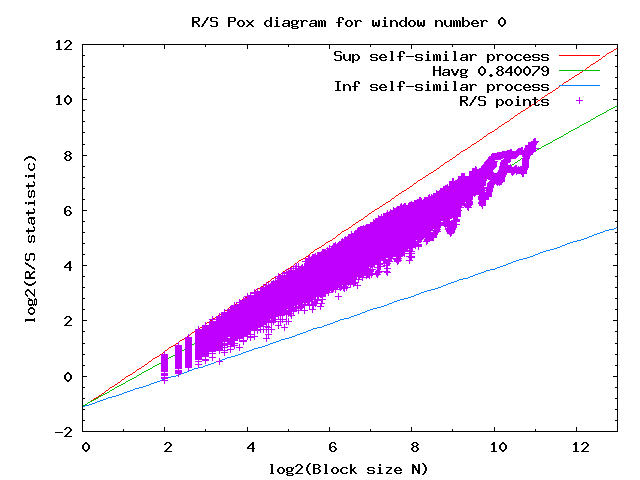
\includegraphics[scale=0.4,type=png,ext=.png,read=.png]{figures/poxdiagram}
\caption{Gr'afica del estad'istico R/S}
\label{fig:poxdiagram}
\end{figure}

En el c'alculo del estimador de Hurst usando el estad'istico R/S, parte del
costo del algoritmo est'a en el c'alculo de $W_k(t_j)$ debido a las repetidas
sumas de los mismo t'erminos. En \cite{Ryuji_Igarashi2007968} se presenta una
forma de mejorar el tiempo de estimaci'on creando una memoria temporal para 
guardar las sumas intermedias. 

\subsection{Gr'aficas varianza-tiempo} \label{subsect:vartime}

El m'etodo de gr'aficas varianza-tiempo, abreviado en este documento
como {\it Var-Tpo}, descrito completamente en \cite{variance-timeplots}, es un
m'etodo que utiliza el gr'afico de $\log (Var(X_k^{(m)}))$ contra $\log (m)$ y luego el m'etodo de m'inimos cuadrados
con los puntos resultantes para obtener una pendiente que es el estimador
$\beta$. El estimador $\beta$ se convierte en un estimador del par'ametro de 
Hurst mediante la f'ormula $H = 1 - \frac{\beta}{2}$. \\

La varianza de la serie agregada se obtiene de la siguiente forma. Para una
serie de tiempo $X_k$ de tama~no $N$ con $ 2 \le m \le \frac{N}{2}$ y un $q$
suficientemente grande de subseries de \{$X_k^{(m)} : k=1,...,q$\} obtenemos la
media de todas las subseries mediante la ecuaci'on (\ref{eq:varmean}) y
calculamos la varianza de cada $m$ particular mediante la ecuaci'on
(\ref{eq:varx}).

\begin{equation} \label{eq:varmean}
\overline{X} = q^{-1} \sum_{k=1}^{q}{X_k^{(m)}}
\end{equation}

\begin{equation} \label{eq:varx}
Var(X_k^{(m)}) = (q -1)^{-1} \sum_{k=1}^{q}{[X_k^{(m)} - \overline{X}]^2}
\end{equation}

La figura \ref{fig:vartimeplot} muestra un ejemplo de la estimaci'on del
par'ametro de Hurst utilizando el m'etodo de gr'aficas de varianza-tiempo. En
esta figura se muestran los puntos resultantes graficados sobre ejes
$\log - \log$ La pendiente resultante debe encontrarse entre las pendientes
$-1 < \beta < 0$, las cuales se muestran en la figura.

\begin{figure}[h]
\centering
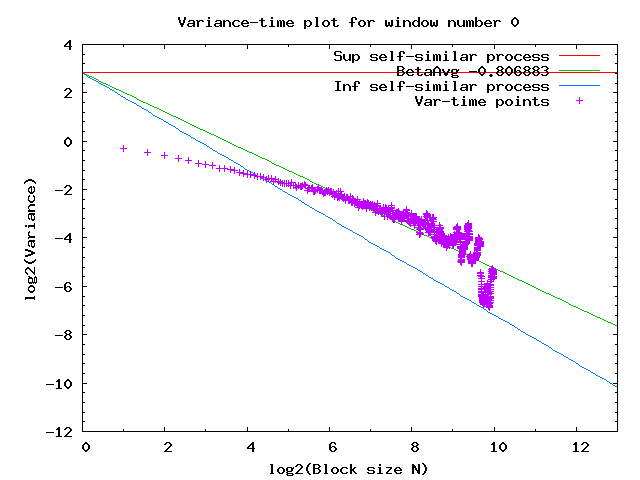
\includegraphics[scale=0.4,type=png,ext=.png,read=.png]{figures/vartimeplot}
\caption{Gr'afica de varianza-tiempo}
\label{fig:vartimeplot}
\end{figure}

\subsection{Varianza modificada de Allan} \label{subsect:mavar}

El m'etodo de la varianza modificada de Allan, denominado {\it MAVAR} por su
nombre en Ingl'es {\it Modified Allan Variance}, es un m'etodo descrito en
\cite{MAVARStefano} que demostr'o tener resultados muy positivos al ser usado
para la estimaci'on del par'ametro Hurst.

Para una serie de tiempo $X_k$ de tama~no $N$, para 
$4 < n \le \lfloor N/3 \rfloor$ se calcula la ecuaci'on principal
(\ref{eq:mavar1}) con la ecuaci'on (\ref{eq:mavarAj}). Los puntos resultantes
son graficados en una gr'afica $\log - \log$ y con los puntos se utiliza el
m'etodo de m'inimos cuadrados. Lo que se obtiene es una pendiente que es el
estimador $\mu$ para el par'ametro de Hurst. $\mu$ est'a relacionado con el
par'ametro de Hurst mediante la f'ormula $H = \frac{\mu}{2} + 2$. La ecuaci'on
(\ref{eq:mavarAj}) se utiliza para minimizar el n'umero de c'alculos obteniendo
un tiempo de corrida $\sim O(N^2)$ \cite{582701}. 

\begin{equation}
\label{eq:mavar1}
\text{Mod } \sigma_y^2 (n c) = \frac{1}{2 n^4 c^2 (N - 3n + 1)} \sum_{j=1}^{N - 3n + 1}{A_j^2(n)}
\end{equation}

\begin{eqnarray}
\label{eq:mavarAj}
A_1(n)  & = & \sum_{i=1}^{n}{(X_{2n+i} - 2X_{n+i} + X_{i})} \nonumber \\
A_{j+1}(n) & = & A_j(n) + (X_{3n + j} - 3X_{2n + j} + 3X_{n+j} - X_{j})
\end{eqnarray}

\begin{figure}[h]
\centering
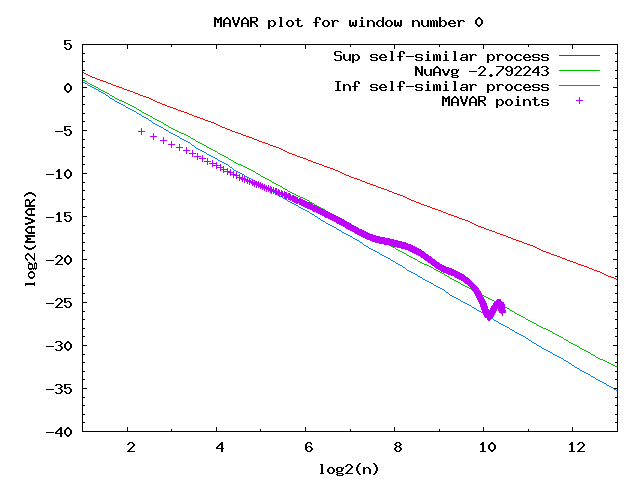
\includegraphics[scale=0.4,type=png,ext=.png,read=.png]{figures/mavarplot}
\caption{Gr'afica de varianza modificada de Allan}
\label{fig:mavarplot}
\end{figure}

La figura \ref{fig:mavarplot} muestra un ejemplo de la estimaci'on del 
par'ametro de Hurst utilizando el m'etodo de varianza modificada de Allan. En la
figura se muestran los puntos resultantes de calcular la ecuaci'on 
(\ref{eq:mavar1}) y graficar los puntos sobre ejes $\log - \log$. La pendiente
resultante, el estimador $\mu$, debe encontrarse entre las pendientes
$-3 < \mu < -2$, las cuales se muestran en la figura.

\section{Problemas con la estimaci'on del par'ametro de Hurst}
\label{sect:problemashurst}

Normalmente lo que se intenta hacer es buscar en los datos caracter'isticas
propias de procesos autosimilares o procesos autosimilares con dependencia de
largo alcance. Debido a que las pruebas para verificar estas caracter'isticas
dependen de valores como el tama~no de la muestra, el intervalo de medici'on e
incluso el m'etodo de estimaci'on utilizado, es m'as razonable hablar de una
estructura autosimilar para una escala y rango particular
\cite{Karagiannis02long-rangedependence:} \cite{Molnar_bottleneckson}.


